\documentclass[journal, a4paper]{IEEEtran}

\usepackage{cite}
\usepackage{graphicx}
\usepackage{url}
\usepackage{amsmath}
\usepackage{minted}

\begin{document}

\title{Analyzing Online Shopping Review Trends}
\author{Eugene Kolodenker, Jose Lemus \\ $\{eugenek, jlemus\}@bu.edu$}
\maketitle

\begin{abstract}
We analyzed 7,824,482 product reviews from Amazon.com's electronics section between the years 1998 - 2013.
Analyzing year to year we answer a few key research questions: 1) Can we observe review quality degrading, 2) Has spam increased, and 3) What other features of reviews have changed year to year? We generated a set of features that focus on both the review text, and the reviewer's activity. With these features we observed user voted helpfulness and, the length of reviews declining. We also see rating inflation, subjectivity increasing, and review polarity becoming more complex. Through clustering we observed reviews shifting towards less helpful, and more biased groups.
\end{abstract}

%%%%%%%%%%%%%%%%%%%%%%%%%%%%%%%%%%%%%%%%%%%%%%%%%%%%%%%%%%%%%%%%%%%%%%%%%%%%%%%%%%%%%%%%%%%%%%%%%%%
\section{Introduction}
The ratings and reviews given to a product have major consequences on how well the product will sell on online websites. Making purchase decisions based on reviews has become a part of the online shopping experience. The quality of an online store can be measured today by the quality of its product reviews. In our analysis we examine the overall shopping experience on the popular website, Amazon, as a subject of the quality of its reviews. Online retailers such as Amazon have much reason to care about the quality of reviews; as customers lose faith in the reviews, these customers may turn elsewhere to do their online shopping. Without helpful, unbiased, and objective reviews shopping experiences suffer, and customers may seek alternatives. By analyzing year-to-year trends we can identify problems, or improvements. Additionally, we are able to analyze if spam, i.e., biased or irrelevant, reviews have increased.

In an ideal world, online product reviews are supposed to help consumers make optimal purchasing decisions. However, product reviews are often times manipulated in order to sway a consumer into buying or not buying the product. This manipulation creates biased and poor reviews. Additionally, as the community changes, review quality may also change. Our project investigates the current state of reviews on Amazon and attempts to identify different types of reviews by taking an unsupervised learning approach.

Various studies have attempted to analyze reviews in the past~\cite{4}. Most of them using supervised or semi-supervised learning. Typically, these studies involve either well labeled data to provide a training set, and a testing set, or involve a lengthy process of manual labeling, i.e., paying students to mark reviews as spam or not spam. Some of them have gone as far as paying for fake reviews to be written to be used for spam classification. While labeled data exists for hotel reviews~\cite{10}, there exists no publicly available good data set for product reviews that contains labeled data. As such, we investigate unsupervised learning through feature engineering and clustering.


%%%%%%%%%%%%%%%%%%%%%%%%%%%%%%%%%%%%%%%%%%%%%%%%%%%%%%%%%%%%%%%%%%%%%%%%%%%%%%%%%%%%%%%%%%%%%%%%%%%
\section{Dataset}
To analyze product reviews we used the Amazon Product Dataset~\cite{1} from Stanford's SNAP. The full dataset consists of 142.8 million reviews (20GB) and spans multiple product categories. These Amazon product datasets are not publicly available. We reached out to Julian McAuley for permission to use these datasets. We initially wanted to analyze this full dataset because it would give us better results. However, processing on this large data set proved to be too challenging, and an exercise in itself of big data analysis. Instead, we worked with what we believe to be a well distributed, and represented category, electronics.

The electronics category contains 7,824,482 reviews and covers the years 1996-2014. The data comes as a list of JSON objects, representing the review. An example can be seen in Figure 1. The reviews consist of unique identifiers for the review author (i.e., reviewer ID), and for the product it was written for (i.e., ASIN). Additionally the review object contains the text, a summary of the text, the time it was written, and the overall rating given to the product. Finally, the reviews contain a "helpful" field that is an array of integers where the first element tells us how many people thought the review was helpful, and the second element tells us the total number of votes.

\begin{figure}[!hbt]
\newminted{c}{fontsize=8}
\begin{minted}[linenos=false]{c}
{
 "reviewerID": "A2SUAM1J3GNN3B",
 "asin": "0000013714",
 "reviewerName": "J. McDonald",
 "helpful": [2, 3],
 "reviewText": "I bought this for my husband who plays the piano. He is having a wonderful time playing these old hymns. The music  is at times hard to read because we think the book was published for singing from more than playing from. Great purchase though!",
 "overall": 5.0,
 "summary": "Heavenly Highway Hymns",
 "unixReviewTime": 1252800000,
 "reviewTime": "09 13, 2009"
}
\end{minted}
\caption{Example review from the Amazon Dataset.}
\end{figure}


Before we began analyzing the dataset, we excluded any reviews that took place in the years of 1996 and 2014. We did this to to analyze the data on a year-to-year basis and data was not collected for the full year in 1996 and 2014. You can see the number of reviews growing year to year in Figure 2. This brought down the size of our dataset to 6,115,878 reviews. Processing these reviews was still not doable locally on consumer laptops. We utilized a 256GB RAM, 16 CPU, Amazon AWS EC2 instance to perform our analysis. Simply loading the data in for analysis took over an hour. The actual analysis takes approximately 6 hours.

\begin{figure}[!hbt]
    \begin{center}
    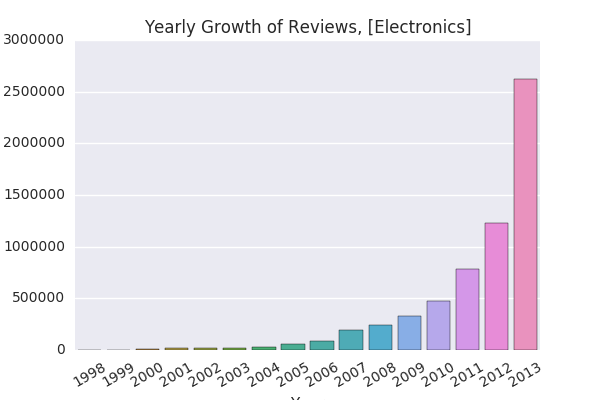
\includegraphics[width=\columnwidth]{yearly_growth_of_reviews.png}
    \caption{Yearly growth of Amazon reviews year to year}
    \end{center}
\end{figure}


%%%%%%%%%%%%%%%%%%%%%%%%%%%%%%%%%%%%%%%%%%%%%%%%%%%%%%%%%%%%%%%%%%%%%%%%%%%%%%%%%%%%%%%%%%%%%%%%%%%
\section{Methods}

\subsection{Feature Engineering}
We set out to analyze the Amazon products dataset for year-to-year trends. In order to understand characteristics of the dataset, first we must derive features. Feature engineering is the process of using domain knowledge to derive characteristics of the data that can then be fed into machine learning algorithms. Feature engineering is a difficult task that is informal, but essential to understanding unlabeled data. It is difficult to fully evaluate the effects of features (i.e., overfitting or underfitting data), so instead we investigated previous work~\cite{4} that leveraged feature engineering to understand review datasets. The literature points to the concept of understanding feature engineering for reviews to either be \textit{review centric}~\cite{2}~\cite{5}, or \textit{reviewer centric}~\cite{6}.
The combination of the two has been shown to be the most effective~\cite{7} and we used this approach.

To analyze the Amazon dataset we built these \textit{review} centric features:
\begin{itemize}
  \item Review length
  \item Percent helpful
  \item Sentiment polarity
  \item Sentiment subjectivity
\end{itemize}

Review length is an important indication of a reviewer's questionable intentions, i.e. spammers, as about 80\% of spammers were found to have no reviews longer than 135 words, while more than 92\% of non-spammers had an average review length greater than 200 words.~\cite{1}.
Seeing this increase or decrease can be an indicator of review quality trend, while also working to answer if spam has increased.

We hypothesize that the lower helpful percentage a review is, the more likely the review is a undesired. This intrinsically true if you assume that the voting peers are unbiased themselves.

By using natural language processing  (NLP) and sentiment analysis we can determine a body of text's polarity, i.e. happiness or sadness towards a product. Additionally, we can determine the review text's subjectivity, i.e. if the review is opinion based, or fact based. We believe that higher quality reviews will be around the global average for polarity (i.e., not overly joyed, but also not overly cynical), and trend towards facts instead of opinion. Opinion based reviews are more likely to be biased.

To analyze the Amazon dataset we built these \textit{reviewer} centric features:
\begin{itemize}
  \item Reviewer's maximum number of reviews on any given day
  \item Reviewer's average given rating
  \item Reviewer's average number of reviews per day
  \item Reviewer's total number of reviews
\end{itemize}

The reviewer's maximum number of reviews on any given day was found to be more than 5 for 75\% of spammers.
While 90\% of identified non-spammers wrote less than a review a day~\cite{1}. This feature is useful in identifying if spam has increased, and marking potential reviews as spam if generated by a spammer.

The reviewer's average given rating can be an indicator of a biased reviewer. If a reviewer provides an above or below global average rating, then they may be more likely to be biased. Additionally, most reviewers have been found to post infrequently. A high number count of average reviews per day may indicate a suspicious user writing fake reviews for products they did not purchase. Similarly, the total number of reviews may indicate a suspicious user.

The actual construction of these features was done using the Python Data Analysis Library (pandas), and the TextBlob library for natural language processing (NLP) and sentiment analysis.

\subsection{Clustering}

To examine if spam has increased, and any other types of reviews (e.g., "helpful, and short", "unhelpful and factual"), we looked at clustering. Because our dataset is unlabeled we took an unsupervised learning approach with the KMeans clustering algorithm. The above features were used in clustering. Other clustering algorithms such as GMM (a probabilistic clustering algorithm) might be more effective in understanding reviews that are a mix of different types, i.e., spam, but also helpful. However, due to resource constraints and the need to perform clustering on approximately 6 million reviews, with up to a dozen features each we would unfortunately run out of time. Instead, we chose the simpler, but efficient, KMeans algorithm.

KMeans suffers from having to choose the number of clusters. Determining this number can be more of an art, than a science. We performed KMeans clustering with varying numbers of clusters, and compared their results with both the inertia (how packed clusters are), and the silhouette score (how similar are members of a cluster). We found the optimal number to be 32 clusters. Unfortunately, at this amount of clusters the data becomes difficult to read. We instead opted to analyze the data at 4 clusters (Figure 7). We believe this smaller number is sufficient to provide us an understanding of 4 major types of reviews.

Typically KMeans clustering is done on geolocated data points, however our product reviews are not. So to be able to represent our clusters in something understand, we utilized Singular Value Decomposition (SVD) to decompose our feature set of 8 down to 2. Its been shown that SVD is an effective way to change KMeans clustering from multi-dimensonal to a two-dimensional problem~\cite{9}.

Finally, to effectively perform accurate clustering, data must be scaled (normalized) to correctly distributed, unit variables. For this, when possible we utilized Scikit Learn's StandardScaler which removes the mean, and scales to unit variance. This was then scaled to be between 0 and 1. When this was not possible, we performed our own scaling by dividing by the maximum. The polarity feature required normalization from (-1, 1) to (0, 1). After this scaling, and SVD we find that KMeans decomposed to percent helpful, and reviewer's average rating as the two major components.


%%%%%%%%%%%%%%%%%%%%%%%%%%%%%%%%%%%%%%%%%%%%%%%%%%%%%%%%%%%%%%%%%%%%%%%%%
\section{Analysis \& Results}
Our analysis of the dataset produced interesting results. Particularly we noticed several review characteristics that we define as essential for unbiased and helpful reviews, declining. However, we do note that the situation is not as grim as previously suspected.

\begin{figure}[!hbt]
    \begin{center}
    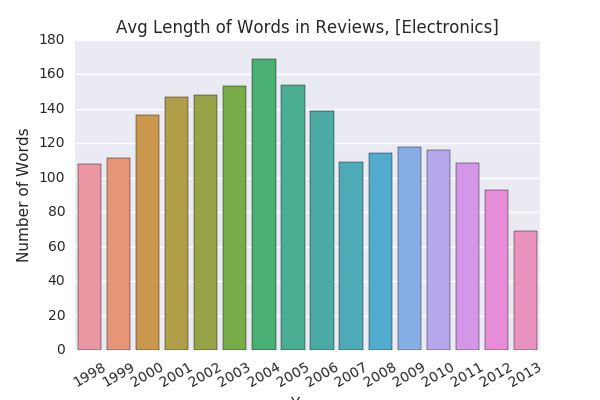
\includegraphics[width=\columnwidth]{avg_length_of_words.png}
    \caption{Average length of review text year to year. Showing rapid decline in recent years, from a peak in 2004.}
    \end{center}
\end{figure}

In Figure 3 we show the year to year average length of review text. We notice a very rapid decline in recent years of review text length. The review text length peaked in 2004, for a reason we do not know. The overall average across the years is 104 words per review, whereas in 2014 it has dropped down to only 60 words per review.

\begin{figure}[!hbt]
    \begin{center}
    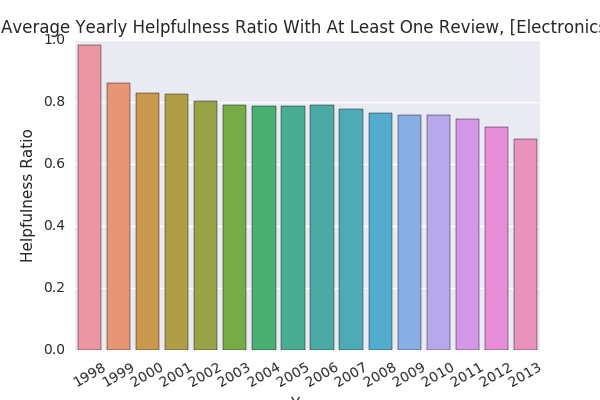
\includegraphics[width=\columnwidth]{helpfulness.png}
    \caption{Average user voted helpfulness of a review year to year. Showing gradual decline for a long period of time now.}
    \end{center}
\end{figure}

In Figure 4 we show the year to year average user voted helpfulness. We take into account only reviews that received at least one vote (either helpful or unhelpful). We note a gradual linear decline from an overall average across the years of 82\% down to 65\%. Reviews are being voted significantly less useful by users today. While this is difficult to causate, it may be potentially good in that users are more vigilant for spam reviews, or it may be bad in that users are seeing more spam than before.

\begin{figure}[!hbt]
    \begin{center}
    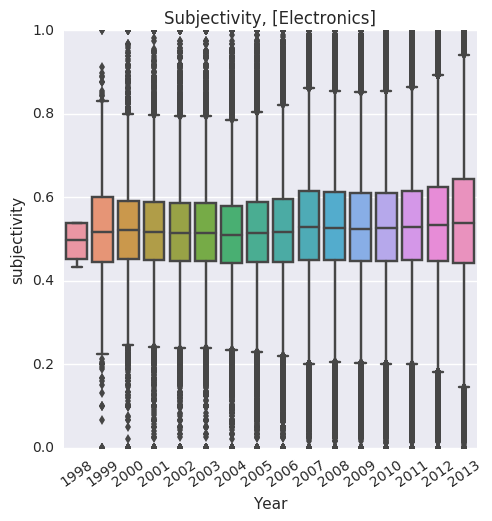
\includegraphics[width=\columnwidth]{subjectivity.png}
    \caption{Subjectivity sentiment analysis on review texts year to year. Showing slow rise in opinion based review text.}
    \end{center}
\end{figure}

\begin{figure*}
  \centering
    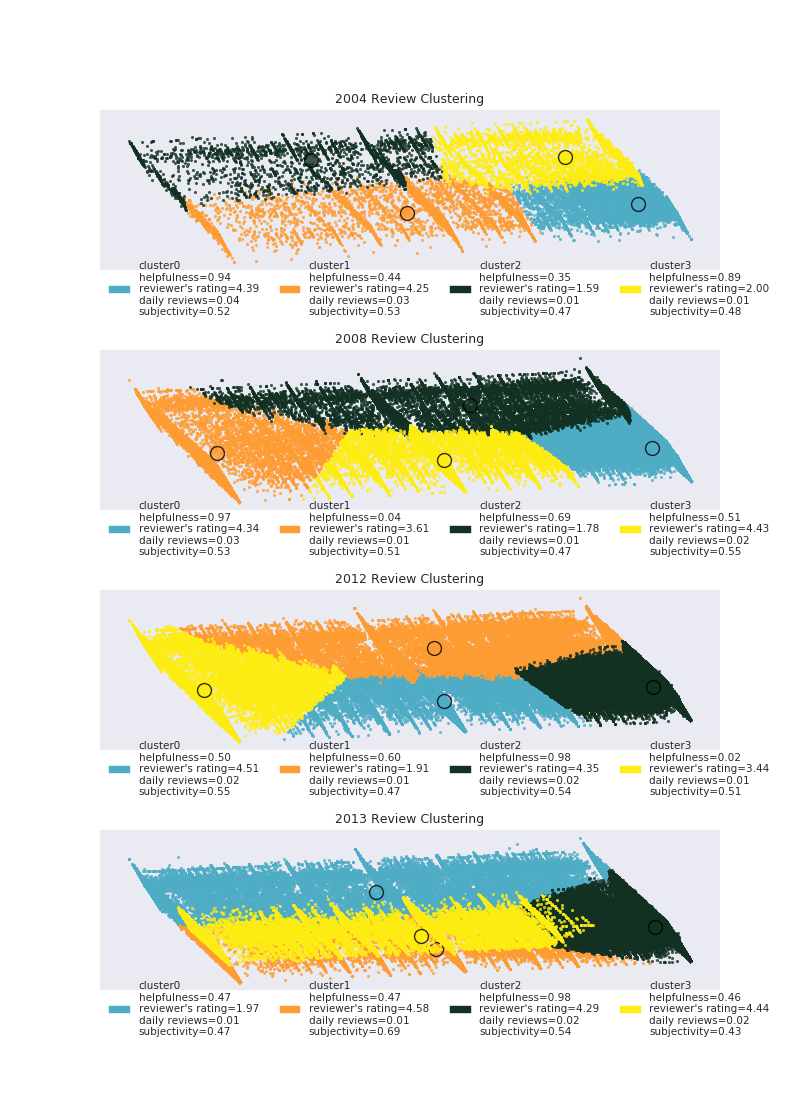
\includegraphics[trim=0 0 0 0,clip,width=.7\textwidth]{clustering.png}
    \caption{KMeans clustering of Amazon reviews.}
\label{fig:overview}
\end{figure*}


\begin{figure}[!hbt]
    \begin{center}
    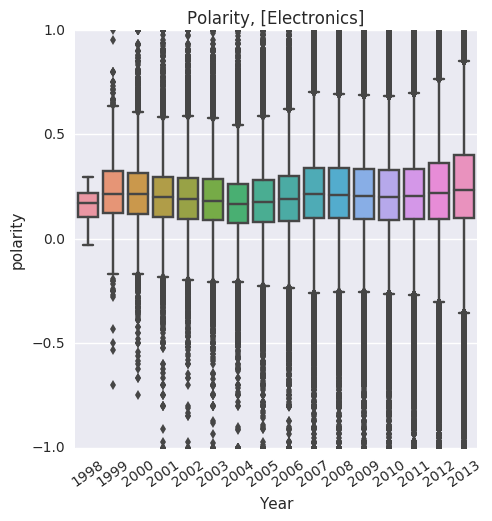
\includegraphics[width=\columnwidth]{polarity.png}
    \caption{Polarity sentiment analysis on review texts year to year. Relatively steady, however potential error is increasing, showing an increase in review text complexity.}
    \end{center}
\end{figure}

Figures 5, and 7 show the results of sentiment analysis on review text. We observe that the subjectivity of reviews is rising slowly. This means that reviews are increasingly becoming more opinion based, and less factual. We believe this to be a poor quality of reviews. The polarity of review text (i.e., if a review is mostly positive sentiment, or negative sentiment) is relatively steady. However, the potential error is increasing year to year. This may be a sign of increasingly complex review text, which is not only difficult for machines to understand, but may be confusing to human readers.


In Figure 6, we show the results of our KMeans clustering analysis. Through dimensionality reduction with SVD, the reviews are able to be plotted on a 2D plot as the result of their two major features, helpfulness, and reviewer's average rating. A highly helpful review can typically be seen as good, while a review where the reviewer's average rating is above the global average can be seen as typically biased.

In 2004, 2008, and 2012, the clustering algorithm identified four types of reviews, that we can name: "helpful and unbiased", "unhelpful and unbiased", "helpful and biased", and "unhelpful and biased". In all four plotted years we see the "helpful and biased" (bottom right) cluster remain the same, with a slightly upward shift. This would indicate the the cluster is becoming less biased, i.e., voting lower on average. Additionally, we notice what used to be the "unhelpful, and unbiased" (2012, far left) cluster drastically shifting in 2013 into a more helpful, but more biased group. This may be an indicator of a transition of people into "paid for review" spammers.


%%%%%%%%%%%%%%%%%%%%%%%%%%%%%%%%%%%%%%%%%%%%%%%%%%%%%%%%%%%%%%%%%%%%%%%%%
\section{Conclusion}
In conclusion through feature engineering, and clustering we are able to analyze trends in Amazon reviews, and identify types of reviews. We are able to note declining helpfulness and review text length, increasing subjectivity, a steady user base that produces helpful and relatively unbiased reviews. The four major types of reviews as determined through clustering remained relatively similar in 2004, 2008, and 2012. However, in 2013 a shift becomes noticeable that indicates the unbiased, but not very helpful cluster becoming much more biased, but also significantly more helpful. This new type of review may be attributable to so called "paid for review" spammers, who write very detailed reviews, but ultimately are paid for them, and biased.

Obtaining useful features to analyze is a challenging task, and even more challenging to choose features that will produce interesting unsupervised learning results. Identifying spam reviews is a difficult task, and without labeled data is extremely difficult to do adequately. A better approach to solely identify spam reviews might supervised learning, such as investing in a month long human study that identifies and creates a set of spam reviews. Those spam reviews can then be used to feed a classifier to essentially automatically find features that describe spam reviews.


%%%%%%%%%%%%%%%%%%%%%%%%%%%%%%%%%%%%%%%%%%%%%%%%%%%%%%%%%%%%%%%%%%%%%%%%%
\begin{thebibliography}{9}
    \bibitem{1}
    Julian McAuley, UCSD, Amazon product data
    \url{http://jmcauley.ucsd.edu/data/amazon/links.html}

    \bibitem{2}
    Shojaee S, Murad MAA, Bin Azman A, Sharef NM, Nadali S (2013) Detecting deceptive reviews using lexical and syntactic
    features. In: Intelligent Systems Design and Applications (ISDA), 2013 13th International Conference on (pp. 53–58). IEEE,
    Serdang, Malaysia

    \bibitem{3}
    Ott M, Choi Y, Cardie C, Hancock JT (2011) Finding deceptive opinion spam by any stretch of the imagination. In: Proceedings of the 49th Annual Meeting of the Association for Computational Linguistics: Human Language Technologies-Volume 1 (pp. 309–319). Association for Computational Linguistics

    \bibitem{4}
    Michael Crawford, Taghi M. Khoshgoftaar, Joseph D. Prusa,  Aaron N. Richter and Hamzah Al Najada,
    Survey of review spam detection using machine learning techniques

    \bibitem{5}
    Jindal N, Liu B (2008) Opinion spam and analysis. In: Proceedings of the 2008 International Conference on Web
    Search and Data Mining (pp. 219–230). ACM, Stanford, CA

    \bibitem{6}
    Li F, Huang M, Yang Y, Zhu X (2011) Learning to identify review spam. In: IJCAI Proceedings-International Joint
    Conference on Artificial Intelligence, vol 22, No. 3., p 2488

    \bibitem{7}
    Jindal N, Liu B (2008) Opinion spam and analysis. In: Proceedings of the 2008 International Conference on Web
    Search and Data Mining (pp. 219–230). ACM, Stanford, CA

    \bibitem{8}
    TextBlob: Simplified Text Processing
    \url{http://textblob.readthedocs.io/en/dev/}

    \bibitem{9}
    Ding, Chris, He, Xiaofeng, K-means Clustering via Principal Component Analysis
    Computational Research Division, Lawrence Berkeley National Laboratory, Berkeley, CA 9472

    \bibitem{10}
    TripAdvisor Data Set
    \url{http://times.cs.uiuc.edu/~wang296/Data/}
\end{thebibliography}

\end{document}

